%% GENERATED by rbrl/gen_figs.py from results/T4_tariff.csv.
%% Do not edit by hand; regenerate.
\begin{figure}[t]
\centering
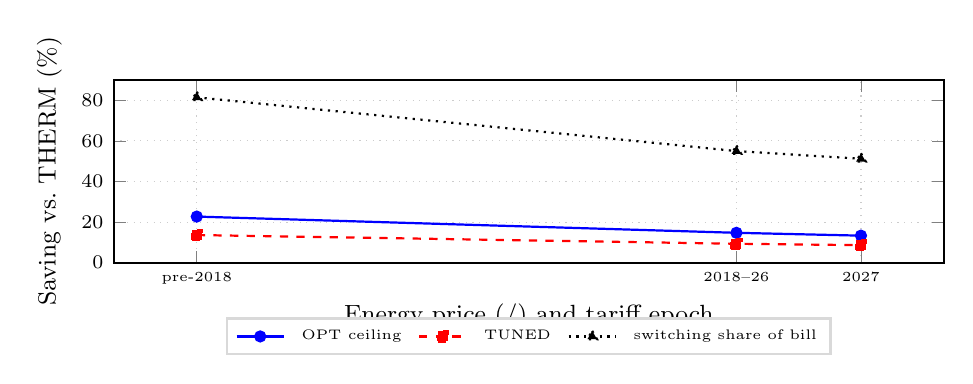
\begin{tikzpicture}
\begin{axis}[
  width=\linewidth, height=3.9cm,
  grid=major, grid style={dotted,gray!40},
  tick label style={font=\scriptsize},
  label style={font=\small},
  legend style={at={(0.5,-0.30)},anchor=north,legend columns=3,
                font=\tiny,draw=gray!30,column sep=4pt},
  thick,
  xtick={0.05,0.18,0.21}, xticklabels={pre-2018,2018--26,2027},
  xticklabel style={font=\tiny},
  xmin=0.03, xmax=0.23,
  xlabel={Energy price (\SAR/\kWh) and tariff epoch},
  ylabel={Saving vs.\ THERM (\%)},
  ymin=0, ymax=90,
]
\addplot[blue,thick,mark=*,mark size=1.8pt]
  coordinates{(0.05,22.7)(0.18,14.7)(0.21,13.3)};
\addlegendentry{OPT ceiling}
\addplot[red,thick,dashed,mark=square*,mark size=1.8pt]
  coordinates{(0.05,13.6)(0.18,9.3)(0.21,8.6)};
\addlegendentry{TUNED}
\addplot[black,dotted,thick,mark=triangle*,mark size=2pt]
  coordinates{(0.05,81.5)(0.18,55.0)(0.21,51.2)};
\addlegendentry{switching share of bill}
\end{axis}
\end{tikzpicture}
\caption{The reported saving is a function of the tariff, not only of the
controller. As the energy price rises, the switching component's share of the
baseline's bill falls from $81.5\%$ to $51.2\%$, and the percentage saved by
the tuned rule and by a clairvoyant schedule falls with it. What the $2018$
reform changed is the denominator, not the quantity recovered: the
\emph{absolute} saving is almost invariant across the three prices
(Section~\ref{subsec:disc_tariff}), so what a scheduler recovers here is a fixed
amount of deferred compressor wear and the percentage moves only because the
bill it is divided into grows. A saving quoted against a pre-reform price is
therefore not comparable with one quoted against the price in force, which
bears directly on the comparison with earlier studies in
Table~\ref{tab:sota}. Held-out
protocol, Riyadh, $\csw=0.15\,\SAR$; identical to
Table~\ref{tab:sensitivity}(a).}
\label{fig:tariff}
\end{figure}
